\documentclass[fr]{../../../../../../eplexam}

\hypertitle{Édification soutenable}{5}{ICAR}{1821}{2018}{Janvier}{Mineure}
{Thibaut Heremans}
{Magali Bodart, Manuel Van Damme et Sophie Trachte}

\section{Hygrothermie et Éclairage}

\subsection*{Question 1 (10pts)}
Un entrepreneur veut lancer une entreprise de titre-service et proposer un service de repassage dans un ancien entrepôt de $50m^2$ de surface et $6m$ de haut. Cinq repasseuses vont travailler 8 heures par jour pendant 230 jours par an avec des centrales vapeur pro qui produisent chacune $1,7kg_v/h$. Les conditions intérieures sont une température de $20^{\circ}C$ et $60\%$ d'humidité relative. Et à l'extérieure on considère une température de $1^{\circ}C$ et $85\%$ d'humidité relative. La masse volumique de l'air à $20^{\circ}C$ est de $\rho_{air}=1,2kg/m^3$.\\

L'installateur du système de ventilation initial installe un système qui a un débit horaire dimensionné de telle manière qu'il permet d'évacuer la production de vapeur des machines. On négligera la transpiration de ces cinq bonne femmes.

\begin{enumerate}
\item Calculer après combien de temps on constatera de la condensation sur les vitrages ($U_{vitr} = 1,0 W/m^2K$) si la ventilation tombe en panne.

\item Quel sera le taux d'humidité relative du local à ce moment là?

\item La toiture (Fig. \ref{toit}) présente-t-elle des risques de condensation interne?
\begin{figure}[h]
\begin{center}
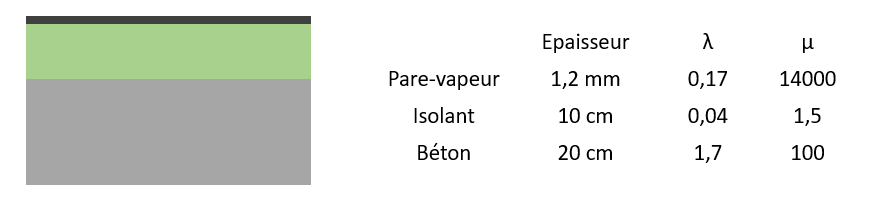
\includegraphics[scale=0.7]{toit}
\caption{Composition du toit de l'entrepôt}
\label{toit}
\end{center}
\end{figure}

\end{enumerate}


\newpage
\subsection*{Question 2 (10pts)}
Vrai(+1) ou faux (-0) :
\begin{enumerate}
\item La couleur des murs d'un local n'a pas d'influence sur le niveau lumineux global du local.
\item La difficulté d'évaluation de l'éclairage naturel provient de la grande variabilité des conditions météo.
\item Pour un ciel couvert CIE, la luminance est indépendante de l'orientation.\item Pour un ciel couvert CIE, la luminance est indépendante de l'altitude du soleil.
\item Concevoir un bâtiment à partir du FLJ va à l'encontre des principes de base de l'architecture bioclimatique.
\item Une protection solaire (contre éblouissement) est toujours plus efficace lorsque placée à l'extérieur.
\item On peut concevoir une bâtiment juste avec le FLJ.
\item L'autonomie dynamique est proportionnelle au temps d'occupation d'un bâtiment lorsque que celui-ci n'est éclairé que naturellement.
\item La couleur apparente d'un objet est indépendante du spectre lumineux de la source qui l'éclaire.
\item Il est possible de calculer le coefficient de réflexion d'une surface simplement à partir de sa luminance et son éclairement.


\newpage
\section{Acoustique}
\subsection*{Question 1 (25\%)}
On souhaite savoir si dans une pièce on dépasse la norme ($<27dB(A)$, $T_0=0,5sec$) Le sonomètre nous fournit $L_{A,eq,30sec}=32dB(A)$ dans la pièce de 8x8x3m. Elle est partiellement meublée et possède un $T=1sec$. Devons nous prendre des dispositions complémentaires?\footnote{Y'avait tout un contexte bizarre mais pour moi faut juste utiliser la formule du formulaire du niveau de pression acoustique standardisé.} Donner 5 solutions pour diminuer le bruit d'une installation de ventilation. 


\subsection*{Question 2 (20\%)}
Dessiner sur un même diagramme de $\alpha_s$ en fonction de la fréquence les courbes de :
\begin{itemize}
\item Laine minérale collée sur un mur lourd
\item Laine minérale + panneau perforé
\item Laine minérale + panneau plein
\item Panneau plein
\end{itemize}


\subsection*{Question 3 (30\%)}
On considère une chambre de $40m^3$ sous un living et on vise le critère acoustique supérieur pour les bruits de chocs. Le plancher est constitué dans l'ordre de plâtre (1000$kg/m^3$, 10mm), d'une prédalle (2500$kg/m^3$, 15cm), d'une chape d'égalisation (1800$kg/m^3$, 70mm), d'une membrane acoustique (26dB), d'une chape (1800$kg/m^3$, 80mm), parquet (600$kg/m^3$, 21mm, R=4dB). La chambre est constituée de 3 murs en blocs de plâtre (1000$kg/m^3$, 10cm) et d'un mur en silico-calcaire (1800$kg/m^3$, 21,5cm).\\
Quel est le $L'_{nTw}$ avant la pose du parquet? Est-ce acceptable?

\subsection*{Question 4 (25\%)}
On sépare du pièce voisine par un doublage de blocs sur membranes. Quel est l'ordre de grandeur du $D_{nTw}$ attendu?\\

Pour finir, on opte pour une autre solution : un doublage par plaques de plâtre. Dessiner une coupe du mur mitoyen ainsi doublé et citer 4 moyens d'améliorer un système à double parois.


\end{enumerate}


 
\end{document}
